\documentclass[12pt]{article}
\usepackage[a4paper, margin=2cm]{geometry}
\usepackage[english]{babel} % To obtain English text with the blindtext package
\usepackage{blindtext}
\usepackage{graphicx} % Required for inserting images
\usepackage{array, multirow} % For extra column formatting
\usepackage{amsmath, amssymb, cancel} %for equation environment
\usepackage{float}
\usepackage{parskip} % For gaps between para
\usepackage{setspace}
\usepackage{pdfpages}
\usepackage{abstract}
\usepackage[export]{adjustbox}
\usepackage{emptypage}
\usepackage{tocloft}
\usepackage[nottoc]{tocbibind}
\usepackage{hyperref, url}
\usepackage[table]{xcolor}
\usepackage{minted}
    \usemintedstyle{monokai}
\usepackage{caption,subcaption}
    \captionsetup{font=footnotesize,labelfont=bf}
    \subcaptionsetup{font=footnotesize}
\usepackage{tcolorbox}
    \newtcolorbox{mintedbox}{
        colback=backcolour,
        boxrule=0pt,
        sharp corners,
        width=\linewidth,
        left=0pt, right=0pt,
        top=3pt, bottom=3pt
    }

\cftsetindents{section}{0em}{2em}
\cftsetindents{subsection}{0em}{2em}

\renewcommand\cfttoctitlefont{\hfill\Large\bfseries}
\renewcommand\cftaftertoctitle{\hfill\mbox{}}

\graphicspath{ {./images/} }

\definecolor{blurple}{HTML}{5865F2}
\definecolor{backcolour}{HTML}{272823}

\hypersetup{
    colorlinks=true,
    linkcolor=black,
    urlcolor=black,
    citecolor=blurple,
}

\urlstyle{same}

\renewcommand{\arraystretch}{1.3}

\setcounter{secnumdepth}{5}
\setcounter{tocdepth}{5}
\newcommand\simpleparagraph[1]{%
  \stepcounter{paragraph}\paragraph*{\theparagraph\quad{}#1}}

%%%%%%%%%%%%%%%%%%%%%%%%%%%%%%%%%%%


\title{PHYC20040 Exp.9 Holography}
\author{Joana Adao}
\date{\today}

\begin{document}

\begin{titlepage}
    \begin{center}

        \begin{figure}[ht]
            
\includegraphics[width=\textwidth]{UCDLogo.png}
        \end{figure}
        
        \begin{figure}
            \centerline{
\includegraphics[width=\paperwidth]{UCDBanner.png}}
        \end{figure}

        \vspace{4cm}

        {\LARGE \bfseries PHYC20090 Electronics and Devices}\\
        \vspace{0.75cm}
        {\Large Experiment No.9 Holography}
        
        \vspace{1cm}
    
    {\Large \textbf{24 February 2025}}

    \vspace{2cm}
    
    {\large \textbf{by Joana C.C. Adao (Student No. 23311051)}}\\
    \medskip
    {\large With Ananya L.}

    \end{center}
    
   \clearpage

\end{titlepage}

\setcounter{page}{1}
\tableofcontents
\pagenumbering{roman}

\newpage

\begin{abstract}
\addcontentsline{toc}{section}{Abstract}
\pagenumbering{arabic}

 
\end{abstract}

%%%%%%%%%%%%%%%%%%%%%%%%%%%%%%%%%%%

\vspace{4cm}

\section{Theory} \label{sec:1}

\subsection{Recording and Reconstruction of Holograms}

Holography is a technique that can record and reconstruct an image based on the "total information" content of the light (wavefronts of light) scattered by the object. These are the basic parameters that describe the light,
wavelength, amplitude, phase, polarisation, and velocity. For holography, only the phase and amplitude of the light are recorded. This process can be understood via Fourier transforms (see §\ref{sec:1.3})
\cite{UCDholo,basicholo1,princetonholo,collier2013optical}.
Visually, the hologram can be described as being as a diffraction screen that diffracts light in such a manner that accurately reconstructs the original object when suitably illuminated
\cite{basicholo1}.
The phase and amplitude information is preserved by a "reference beam" and its interference with the light being reflected off the object's surface
\cite{UCDholo,princetonholo}.

\textbf{Recording} a hologram requires the presence of the "object beam", which illuminates the object and reflects onto the recording material (typically an emulsion photographic plate for optical holography), and the
"reference beam", the light from an apparent source that shines directly onto the recording material
\cite{UCDholo,basicholo1} (see Figure \ref{fig:1}).
These beams interfere to create an interference pattern that is recorded onto the recording material (see Figure \ref{fig:2}). Precise positioning of the laser source, beam splitter, mirrors, and emulsion photographic plate is necessary as it determines the
fringe spacing of the interference pattern. Therefore misalignmnets affect the clarity and resolution of the final hologram
\cite{UCDholo,collier2013optical}.

\begin{minipage}{.49\textwidth}
    \captionsetup{hypcap=false}
    \centering
    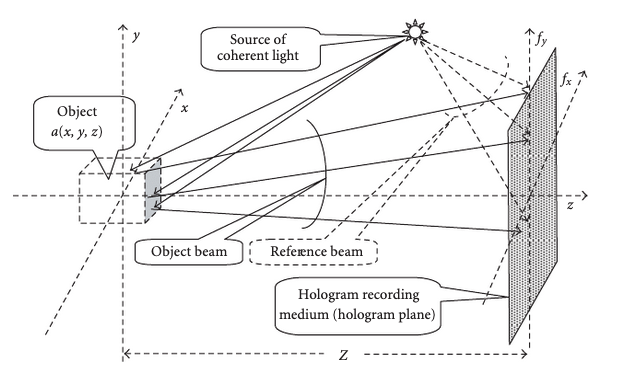
\includegraphics[width=\linewidth]{hologram construction.png}
    \captionof{figure}{\centering sample caption \protect\cite{holoimg1}.}
    \label{fig:1}
\end{minipage}
\hfill
\begin{minipage}{.49\textwidth}
    \captionsetup{hypcap=false}
    \centering
    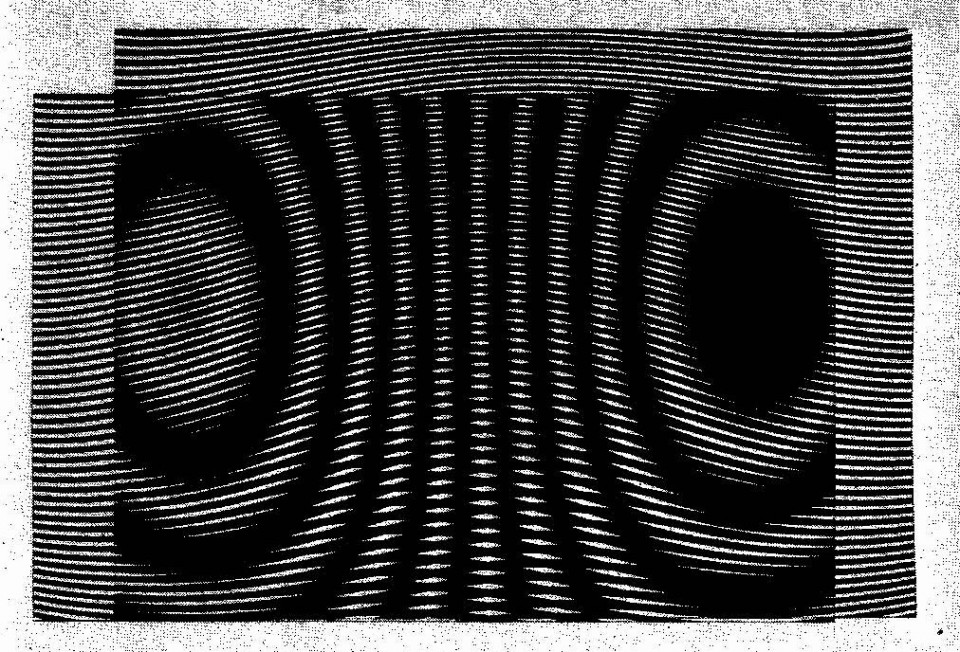
\includegraphics[width=\linewidth]{holo interference.jpg}
    \captionof{figure}{\centering sample caption \protect\cite{kafri1990physics}.}
    \label{fig:2}
\end{minipage}

\textbf{Reconstructing} a hologram is through diffraction, and it is found that the spacing of the interference fringe are of the correct size (typically between 0.4 to 0.7 microns) to give the desired diffratcion effects 
\cite{UCDholo}.
The resulting wave structure is then identical to the original, a reconstruction of the original object in 3D detail.
A "reconstructing beam", typically the original source reference beam or light of similar coherency, illuminating the photographic plate in the direction of the original source is what allows one to be able to see the hologram
\cite{UCDholo}.
The reconstructed can be seen moving through parallax effects when the angle of viewing is shifted. The existence of this parallax is what indicated whether the object has three-dimensions \cite{UCDholo}.

\subsection{Amplitude and Phase} \label{sec:1.2}

Tradiotional photography methods differ from holography in the sense that with holography the phase information is also retrieved, unlike photography where only spatial distribution of light intensity (amplitude) is considered which
is averaged over all phases of light \cite{collier2013optical}.

The \textbf{amplitude} of a wave is defined as the max displacement of the wave \cite{britlight}.
For a hologram the amplitude variations will affect primarily the contrast of the recorded interference pattern, influencing the final hologram quality \cite{UCDholo,latychevskaia2009simultaneous}.
Most hologram reconstruction methods assume pure amplitude, but most real-life objects affect amplitude scattering and are therefore wavelength-dependent, 
meaning amplitude is essential for accurate holographic image reconstructions \cite{latychevskaia2009simultaneous}.

The \textbf{phase} of a wave determines where the electric field is in an oscillation cycle \cite{Paschotta_2018_optical_phase}.
The optical wave can be described with a phasor (complex amplitude), which relates the optical phase to the complex phase. 
A plane wave propagating in the z-direction can be described with $Ae^{i(\omega t - kz)}$ (see §\ref{sec:1.3}).
Interference strongly depends on optical phases \cite{Paschotta_2018_optical_phase}.
It is the phase encodement that makes a hologram appear to have a three-dimensional structure due to the phase differences in the interference pattern \cite{Paschotta_2018_optical_phase}.

\begin{figure}[H]
    \centering
    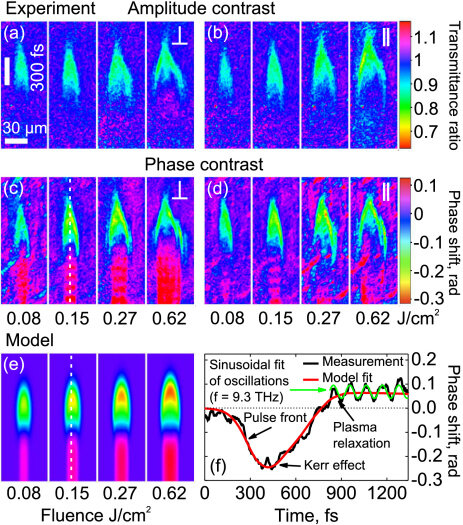
\includegraphics[width=.5\textwidth]{amplitude v phase contrast.jpg}
    \caption{\centering Comparison of amplitude (a-b) and phase (c-d) contrast in holography. Modeled phase images (e) and cross-sections (f) of experimental (c) phase images \protect\cite{ampvphaseimg}.}
    \label{fig:6}
\end{figure}

The difference between the amplitude and phae contrasts in holography are depicted in Figure \ref{fig:6}, comparing the experimental (a-d) and modeled (e) reconstructions.
Amplitude contrast images (3a-b) show variations in intensity (amplitude) which affects the trasmittance ratio, while phase contrast images (3c-d) show variations in phase (phase shifts), affecting the structural reconstruction accuracy \cite{latychevskaia2009simultaneous,ampvphaseimg}.
The modeled image (3e) illustrates how amplitude and phase contribute to the final reconstruction of the holographic image, with the phase graph (3f) showcasing the spatiotemporal evolution of the phase shift \cite{ampvphaseimg}.

\subsection{Fourier Transforms} \label{sec:1.3}

Consider the reflected waves as seen in Figure \ref{fig:3}. The detailed nature of this "object beam" is dependent on the object's shape and surface
characteristics. Taking a general approach, describe the object beam as a superposition (combination) of plane waves,

\vspace{-2ex}
\begin{gather*}
    \psi_0 (r,t) = A_0 \iint F_0 (k_x,k_y) e^{i(\omega t- k_x x- k_y y - k_z z)} dk_x dk_y 
\end{gather*}

where $(k_x^2 + k_y^2 + k_z^2)^{1/2} = k = \lambda / 2$. Suppose we have permitted this wave $\psi_0$ to interfere with a reference beam given by

\vspace{-2ex}
\begin{gather*}
    \psi_1 (r,t) = A_1 e^{i(\omega t - kz)}
\end{gather*}

and have recorded the resulting intensity pattern on a photographic plate positioned in the plane $z = 0$. The intensity recorded on the plate is then

\vspace{-2ex}
\begin{gather*}
    I(x,y) = \lvert A_1 + A_0 \iint F_0 (k_x,k_y) e^{-i(k_x x + k_y y)} dk_x dk_y \rvert^2
\end{gather*}

Expanding the right-hand side of this equation, we will have terms proportional to $\lvert \psi_0 \rvert^2$, $\lvert \psi_1 \rvert^2$, and $\lvert \psi_0 \psi_1^* \rvert$.

Assuming that the reference beam is much more intense than the object beam (ie. $\lvert \psi_1 \rvert \gg \lvert \psi_0 \rvert$), then the term in $\lvert \psi_0 \rvert^2$ can be ignored,
and the intensity can be approximated as

\vspace{-2ex}
\begin{gather*}
    I (x,y) \approx \lvert A_1 \rvert^2 + A_0 A_1^* \iint F_0 (k_x,k_y) e^{-i(k_xx + k_yy)} dk_x dk_y + A_1 A_0^* \iint F_0 (k_x,k_y) e^{+i(k_xx + k_yy)} dk_x dk_y
\end{gather*}

The transmission function for a developed plate can be expressed as $T(x,y) = 1 - \gamma I(x,y)$ where $\gamma$ is a function of the exposure and
developing processes. Therefore, the hologram's transmission function is

\vspace{-2ex}
\begin{gather*}
    T(x,y) = C_0 - \gamma A_0A_1^* \iint F_0 (k_x,k_y) e^{-i(k_xx+k_yy)} dk_x dk_y - \gamma A_1 A_0^* \iint F_0 (k_x,k_y) e^{+i(k_xx +k_yy)} dk_x dk_y
\end{gather*}

where $C_0$ is a constant. Essentially, the hologram contains both scaled versions of the two-dimensional Fourier tranform of the object beam and its inverse, superimposed on each other.
When this hologram is illuminated with a plane wave life the originall reference beam, another Fourier transformation occurs, which leads to

\vspace{-2ex}
\begin{gather*}
    \psi (r,t) = \iint F(k'_x,k'_y) e^{i(\omega t - k'_xx - k'_yy - k'_zz)} dk'_x dk'_y
\end{gather*}

where, according to Fourier optics,

\vspace{-2ex}
\begin{gather*}
    F(k'_x,k'_y) = \left( \frac{1}{2 \pi} \right)^2 \iint T(x,y) e^{i(k'_xx + k'_yy)} dxdy
\end{gather*}

The three terms that make up $T(x,y)$ obligingly integrate as delta functions (unlike the ignored $\lvert \psi_0 \rvert^2$ term, which would not behave as such), and we find

\vspace{-2ex}
\begin{gather*}
    F(k'_x,k'_y) = - \gamma A_1^* A_0 F_0 (k'_x,k'_y) - \gamma A_1 A_0^* F_0^* (-k'_x, -k'_y) + C_0 \delta (k'_x)\delta(k'_y)
\end{gather*}

As a result, when the hologram is illuminated correctly (as in Figure), the emerging wave consists of three parts: (left) a term that is proportional to the original object beam, effectively
reconstructing the object in all details of amplitude and phase; (centre) a so-called "twin reconstruction" or "twin image", which can be shown to be the original object beam, reflected across the
photographic plate and travelling backwards in time; and (right) an undeflected segment of the reference beam travelling along the z-axis.

\begin{figure}[H]
    \centering
    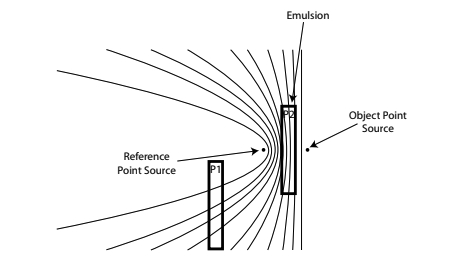
\includegraphics[width=.5\textwidth]{holography1.png}
    \caption{\centering Two-dimensional projection of the interference patterns produced. A photographic plate at P1 would result in a transmission hologram.
    A photographic plate at P2 wiuld result in a reflection hologram. \protect\cite{princetonholo}}
    \label{fig:3}
\end{figure}

\subsection{Properties of Laser Light in Holography}

Holography relies on the properties of laser light in order to reconstruct and record the necessary three-dimensional images. Lasers are \textbf{highly monochromatic, coherent, intense, and coherent} which allows for stable
interference patterns. These properties are then what enable the precise encoding of the phase and amplitude information necessary for the reconstruction of the hologram \cite{UCDholo}.

\subsubsection{Monochromaticity}

For stable interference the source itself must be stable such that the light is emitted at a single wavelength \cite{princelaser}.
Any variation in wavelength would cause the recorded fringes to become "blurred", which affects the clarity of the final hologram, so the laser being monochromatic ensures the fringes remain sharp and stable (well-defined).

\begin{figure}[H]
    \centering
    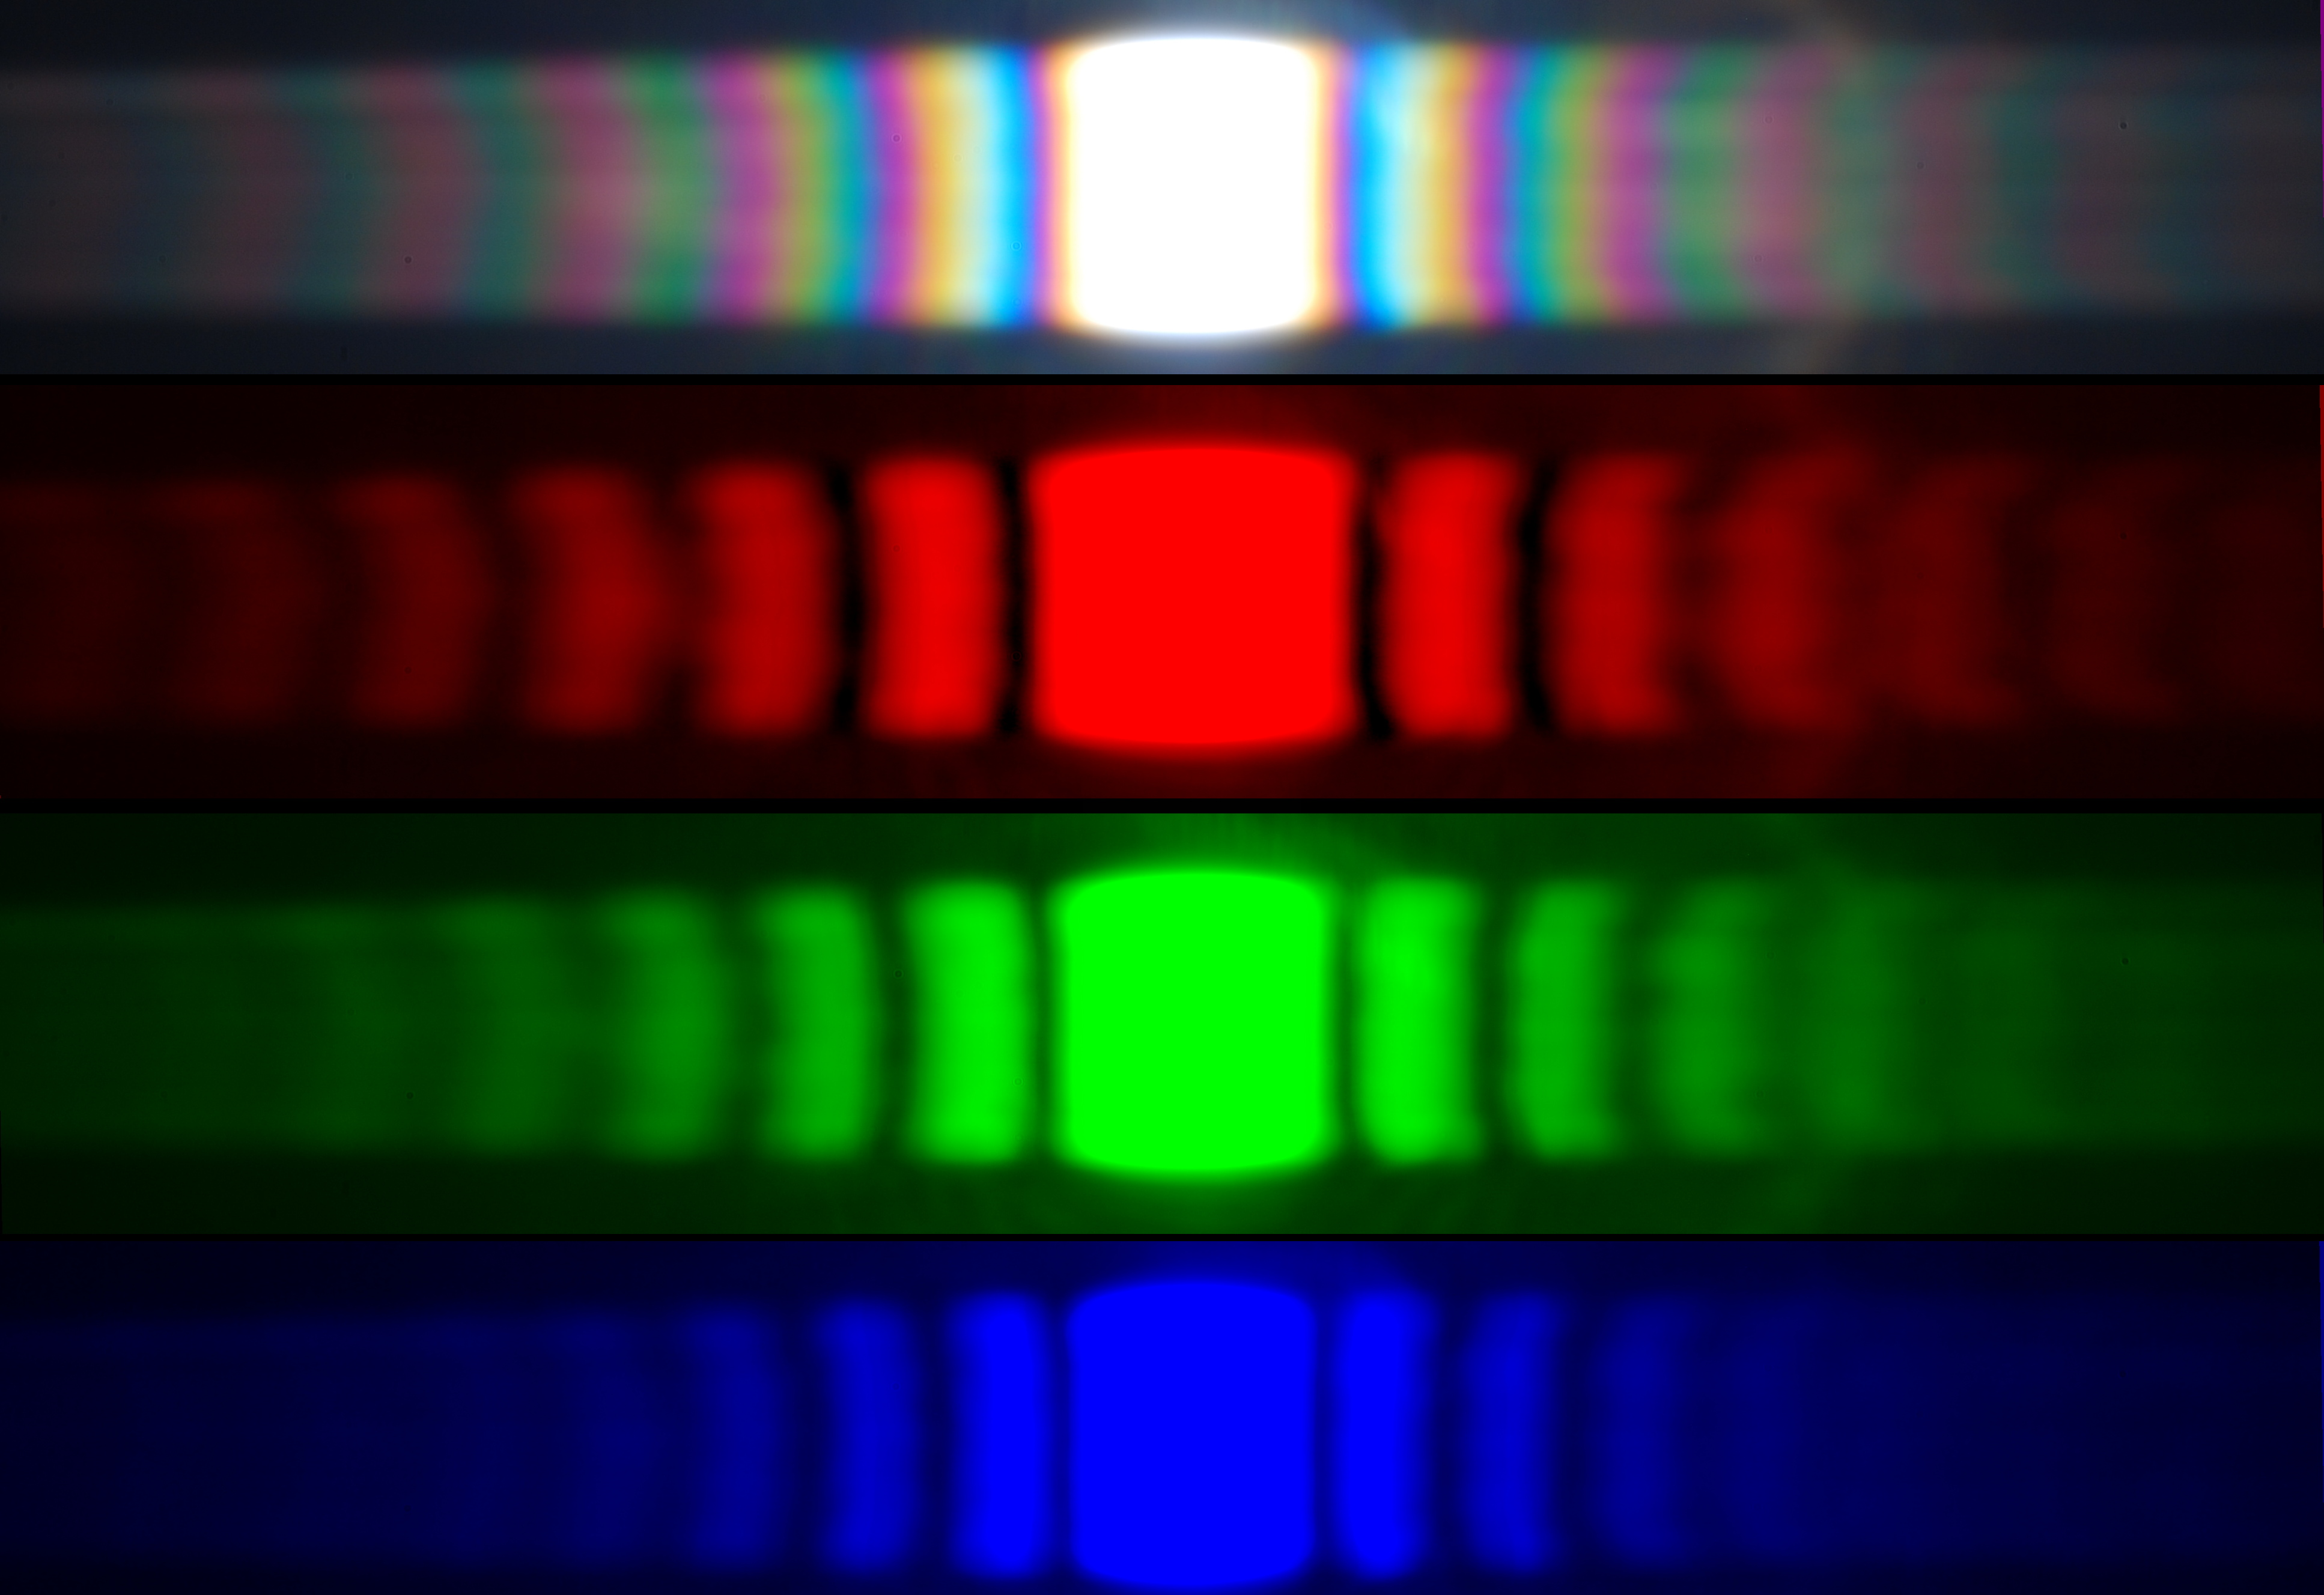
\includegraphics[width=.5\textwidth]{interference patterns.jpg}
    \caption{\centering sample caption \protect\cite{holoimg2}.}
    \label{fig:4}
\end{figure}

As can be seen in Figure \ref{fig:4}, the interference patterns from the monochromatic light sources (red, green, blue) appear much sharper than the "blurred" interference pattern of the white light (top)
due to the range of wavelengths present in white light.

\subsubsection{Coherence}

For there to be stable interference the light source must have a fixed phase relationship at different points in time and/or space \cite{wolf2007introduction}.
This property ensures that the reference and object beams maintain a consistent phase difference, allowing them to interfere and create the fringes of greater and lesser amplitudes
\cite{Born_Wolf_Bhatia_Clemmow_Gabor_Stokes_Taylor_Wayman_Wilcock_1999}.
Thus, lasers are used in holography due to their spatial, strong correlation between electric fields at difference points in the beam profile, and temporal, strong correlation between electric fiels at one point at different times, coherences
\cite{Paschotta_2007_coherence} which results in high-quality holographic images.

\begin{figure}[H]
    \centering
    \begin{subfigure}[b]{.45\textwidth}
        \centering
        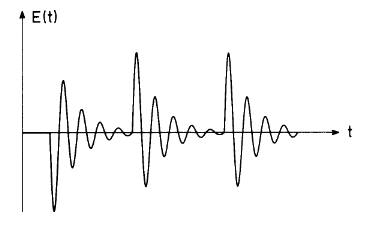
\includegraphics[width=\linewidth]{incoherent source.png}
        \caption{\centering Incoherent lamp light source}
        \label{fig:5a}
    \end{subfigure}
    \hfill
    \begin{subfigure}[b]{.45\textwidth}
        \centering
        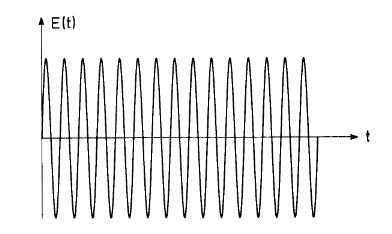
\includegraphics[width=\linewidth]{coherent source.png}
        \caption{\centering Coherent laser light source}
        \label{fig:5b}
    \end{subfigure}
    \caption{\centering '(a) The electric field strength E(t) of light of a lamp consists of uncorrelated individual wave tracks.
    (b) Laser light consists of a single coherent very strong wave track.' \protect\cite{haken1986laser}.}
    \label{fig:5}
\end{figure}

A graphical representation of an incoherent (\ref{fig:5a}) and a coherent (\ref{fig:5b}) can be seen in Figure \ref{fig:5} above. Visually, it can be understood why a coherent
source is necessary for the production of a hologram.

\subsubsection{Intensity and Directionality}

Laser light possesses both high intensities and high directionality, such laser light does not diffract or spread out like other conventional light sources.
High intensities ensure an interference pattern with high contrast and thus the visibility of the final holographic image \cite{kafri1990physics,haken1986laser}.
The high directionality of the laser source allows for percision over the angles and positioning of the reference and object beams, allowing for the accurate recording of the hologram.

\subsection{Types of Optical Holograms}

Optical holography is the recording and reconstruction of a hologram using laser light on a holographic plate and demands the presence of a real object in a highly stable and vibration-free
recording environments for optimal encoding \cite{basicholo1}.
The most common types of optical holograms are transmission and reflection holograms.

\begin{figure}[H]
    \centering
    \begin{subfigure}[b]{.45\textwidth}
        \centering
        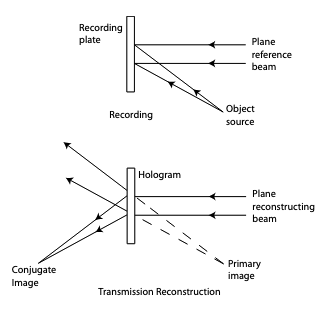
\includegraphics[width=\linewidth]{transmission reconstruction.png}
        \caption{\centering Transmission reconstruction}
        \label{fig:9a}
    \end{subfigure}
    \hspace{-1em}
    \begin{subfigure}[b]{.45\textwidth}
        \centering
        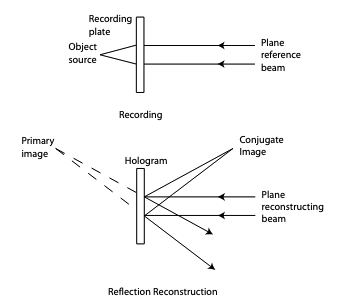
\includegraphics[width=\linewidth]{reflection reconstruction.png}
        \caption{\centering Reflection reconstruction}
        \label{fig:9b}
    \end{subfigure}
    \caption{\centering Recording and reconstruction setups for (\subref{fig:9a}) transmission and (\subref{fig:9b}) reflection holograms \protect\cite{princetonholo}.}
    \label{fig:9}
\end{figure}

\subsubsection{Transmission Holograms}

Transmission holograms require a monochromatic reconstructive beam (laser) or a single frequency source. This limitation is due to the way the hologram stores its information \cite{princetonholo}.
See the position of the photographic plate at P1 in Figure \ref{fig:3} and how the interference patterns are produced on that plate.
For a transmission hologram the interference is observed to be recorded \textit{perpendicular} to the plane of the photographic plate. Due to this, any frequency of light can then
pass through the plate, creating a washed-out appearance of the holograms as every frequency of light subsequently forms an image \cite{princetonholo}.

\begin{figure}[H]
    \centering
    \begin{subfigure}[b]{.43\textwidth}
        \centering
        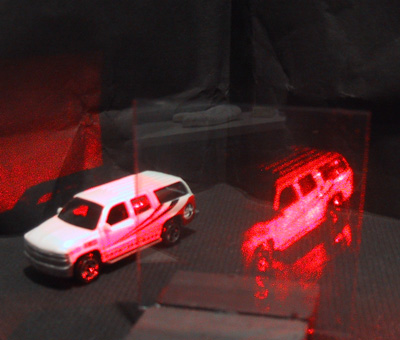
\includegraphics[width=\linewidth]{transmission holo.jpg}
        \phantomcaption
    \end{subfigure}
    \hfill
    \begin{subfigure}[b]{.55\textwidth}
        \centering
        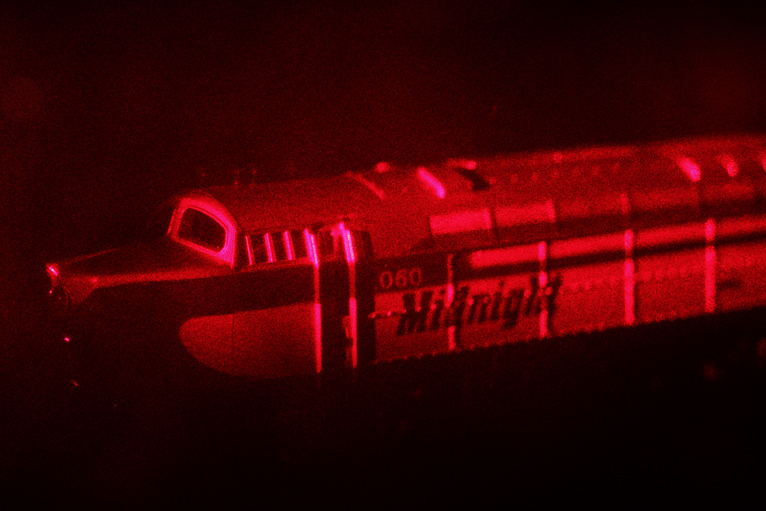
\includegraphics[width=\linewidth]{trans 2 holo.jpg}
        \phantomcaption
    \end{subfigure}
    \caption{\centering Two transmission holograms, seen with red laser light \protect\cite{transholo,reftransholo}.}
    \label{fig:7}
\end{figure}

\subsubsection{Reflection Holograms}

Reflection holograms obtained their name due to the fact that they reflect a reconstruction of the object beam to form an image rather than transforming the reconstructive beam into a replica of the object beam \cite{princetonholo}.
See the position of the photographic plate at P2 in Figure \ref{fig:3} and how the interference patterns are produced on that plate.
For a reflection hologram the interference pattern is observed to be recorded \textit{parallel} to the plane of the photographic plate and along the thickness of the emulsion which is essential to reflection holograms (but irrelevant to transmission holograms) \cite{princetonholo}.
Reflection holograms, unlike transmission holograms, can be seen under white light and thus are also commonly referred to as "white-light holograms".

\begin{figure}[H]
    \centering
    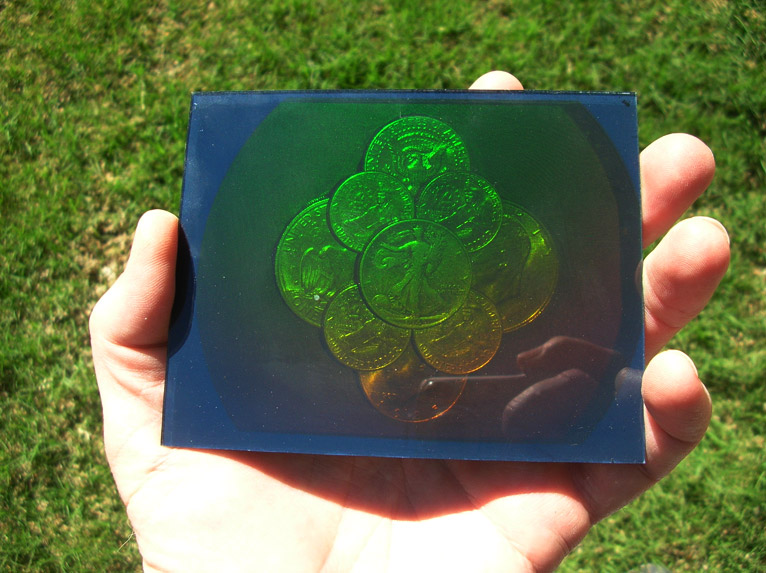
\includegraphics[width=.5\textwidth]{reflection hologram.jpg}
    \caption{\centering A reflection hologram, seen under sunlight \protect\cite{reftransholo}.}
    \label{fig:8}
\end{figure}

bragg diffraction or something idk im mad tired rn

\subsection{How Shape, Design and Dimension Affect the Hologram}


\subsection{Applications of Holography}




\section{Methodology} \label{sec:2}



\section{Results and Calculations} \label{sec:3}



\newpage

\section{Conclusion} \label{sec:4}



\newpage

%%%%%%%%%%%%%%%%%%%%%%%%%%%%%%%%%%%

\bibliographystyle{IEEEtran}
\bibliography{References} \label{sec:ref}

\vspace{1.5cm}

\listoffigures

\listoftables


\end{document}